% Expanded mathematical manuscript based on MATH.md and the frozen experiment protocols.
% This TeX source now contains technical material beyond the shorter Markdown summary.
% Standalone source: no external bibliography, figures, or included project files required.
\documentclass[11pt]{article}
\usepackage[T1]{fontenc}
\usepackage[utf8]{inputenc}
\usepackage{lmodern}
\usepackage[margin=1in]{geometry}
\usepackage{amsmath,amssymb,amsthm}
\newtheorem{proposition}{Proposition}[section]
\newcommand{\E}{\mathbb{E}}
\newcommand{\Var}{\operatorname{Var}}
\newcommand{\Cov}{\operatorname{Cov}}
\newcommand{\KL}{D_{\mathrm{KL}}}
\newcommand{\sg}{\operatorname{stopgrad}}
\usepackage{booktabs,tabularx,array}
\usepackage{pgfplots}
\pgfplotsset{compat=1.18}
\usepackage{microtype}
\usepackage{xurl}
\usepackage[colorlinks=true,linkcolor=blue,urlcolor=blue]{hyperref}
\hypersetup{pdftitle={Reward variation without demonstrated token savings: an audited exploratory study},pdfauthor={Arya Somu}}
\setlength{\emergencystretch}{2em}
\title{Reward variation without demonstrated token savings:\\an audited exploratory study}
\author{Arya Somu}
\date{Working paper draft: October 10, 2026}
\begin{document}
\maketitle

The exploratory fixed-reward comparison is complete and independently audited. It found a small, uncertain response without a token-cost reduction. This working paper preserves the mathematical derivations and all failed attempts; adaptive reward superiority and generalization remain unestablished. Public release remains subject to review.

\begin{abstract}

We study whether reinforcement learning with a configurable token-cost penalty can steer a small coding model toward different success-cost preferences. The task is simulated expression repair, with restricted candidate selection and hidden-example scoring. We derive an adaptive penalty update relative to a fixed initial policy and distinguish its ideal constrained objective from the finite-sample LoRA training procedure. An independently audited, one-seed fixed-reward continuation compares success-only reward with success minus generated-token cost divided by 1,024. Both arms receive 64 groups of four fresh trajectories. On 32 reused development tasks with two matched samples each, the cost-penalty arm scores 54/64 versus 52/64 while averaging 1,567.89 versus 1,556.69 generated tokens. The paired cost difference is +11.20 tokens (descriptive 95 percent task interval: -65.09 to +88.34); the accuracy difference is +3.125 percentage points (-6.25 to +14.06). Thus this horizon does not demonstrate a token-cost reduction or a reliable accuracy gain. Retrospective reconstruction finds 59 penalty updates versus 30 success-only updates: length variation activates 33 penalty groups with homogeneous success. Every active update is gradient-clipped. Identical first-group trajectories illustrate how reward variation can activate learning without guaranteeing later token savings. Completed earlier pilots include a fixed/adaptive tie and failed sensitivity diagnostics. Encrypted recovery and strict deterministic restart qualification enabled collection after two historical interruptions; the reused control has different determinism settings. One seed, repeatedly inspected development data and this execution difference limit interpretation. A prospective matched multi-seed held-out study is required for adaptive-steering or generalization claims.

\end{abstract}
\section{Introduction}

Model capability is often reported independently of inference cost. For a deployed policy, both solve probability and generated computation matter. A linear utility, \(R=S-\lambda C\), makes that preference explicit, but a fixed penalty does not directly specify the direction of improvement relative to an initial policy.

\href{https://anishlk.com/swe-2-extended/}{Lakkapragada} proposes adapting the penalty to balance relative success gains and cost reductions. His controlled environment has five trainable parameters and a known success-cost relationship. Our question is how this idea behaves when the policy is a language model trained through a small LoRA adapter, with variable-length sampled reasoning and stochastic optimization.

We separate three questions: whether the numerical estimator is faithful to the sampled policy; whether a fixed cost preference produces an observable behavioral response; and whether adaptive preferences steer that response on untouched tasks across training seeds. Each requires different evidence. Infrastructure correctness and improved prompting alone do not answer the final question.

Our contribution is a transparent mathematical account and an audited exploratory finding, including failed diagnostics and interruptions. We do not claim a new reward algorithm or a superior coding policy. REINFORCE-style language-model optimization has prior empirical support in other alignment settings~\cite{rloo}. Work on length penalties also identifies optimization and sparse-signal issues~\cite{dler}; its tasks and training recipe differ from ours. Those results motivate examining the estimator and optimizer, not transferring their reported gains to this experiment.

\section{Objective and adaptive update}
\label{sec:objective}

This section supplies the complete interior derivation of the controller adapted from \href{https://anishlk.com/swe-2-extended/}{Lakkapragada}. It is an ideal policy-space construction. The current exploratory training run tests two \emph{fixed} utilities; an adaptive experiment remains prospective.

\subsection{Reader's guide and mathematical prerequisites}

The intended baseline is elementary probability, derivatives, and matrix multiplication. We use natural logarithms throughout. $\E[U]$ denotes an average over the specified random experiment; $\Var(U)=\E[(U-\E U)^2]$ and $\Cov(U,V)=\E[(U-\E U)(V-\E V)]$. A gradient $\nabla_\theta f$ collects the partial derivatives of a scalar $f$ with respect to the trainable parameters $\theta$. A conditional expectation holds the variables following the conditioning bar fixed. The symbol $\widehat{\phantom{u}}$ marks an estimate computed from observations. An $\operatorname*{arg\,min}$ returns a minimizing argument, whereas $\min$ returns the minimum value.

The derivation follows this chain: specify a common success--cost improvement; rewrite its two constraints as a minimum; express that minimum using a mixture weight; identify the corresponding linear reward; solve one regularized mixture update; estimate the reward gradient from discrete samples; apply it through LoRA and the optimizer; and compare complete final-policy evaluations. Equations describe these transitions explicitly. They do not supply a closed-form solution for the trained language model.

\begin{center}
\small
\begin{tabularx}{\linewidth}{@{}lX@{}}
\toprule
Symbol & Meaning \\
\midrule
$x,e,y$ & Task, effort condition, and generated trajectory \\
$\pi,\theta$ & Policy distribution and its trainable adapter parameters \\
$S,C,s,c$ & Realized success/cost and their policy expectations \\
$s_0,c_0,u,v$ & Fixed baseline expectations and relative improvements \\
$\tau,\alpha,\beta,\lambda,\eta$ & Common improvement, preference, dual mixture, token penalty, controller step size \\
$G,i,A_i,h_i$ & Training-group size, sample index, advantage, trajectory score gradient \\
$k,t$ & Completed training-group count and actual optimizer-update count \\
$N,M,j,m$ & Evaluation tasks, samples per task, task index, sample index \\
$B$ & Bootstrap replicate count; in Appendix~\ref{sec:cachegradient}, a separately local computation-block count \\
\bottomrule
\end{tabularx}
\end{center}
The LoRA matrices also use $A,B$; those matrix symbols are distinct from sampled answer $A$, scalar advantage $A_i$, and bootstrap count $B$. Their types and subscripts identify their roles. Subscript $e$ is omitted when one effort condition is held fixed. Later proofs invoke the ordinary product/chain rules, finite-sum differentiation, and independence; the transformer architecture and these elementary calculus rules are prerequisites rather than new results proved here.

\subsection{Probability space, baseline and units}

Let $X\sim D_e$ be a task at effort condition $e$, and let $Y$ be a generated trajectory under policy $\pi$. The hidden-example evaluator produces $S(X,Y)\in\{0,1\}$; generated-token cost is $C(Y)\geq0$. Define
\begin{align}
 s_e(\pi)&=\E_{X\sim D_e,\,Y\sim\pi(\cdot\mid X,e)}[S(X,Y)],\label{eq:success}\\
 c_e(\pi)&=\E_{X\sim D_e,\,Y\sim\pi(\cdot\mid X,e)}[C(Y)].\label{eq:cost}
\end{align}
The original policy $\pi_0$ fixes $s_{e,0}=s_e(\pi_0)>0$ and $c_{e,0}=c_e(\pi_0)>0$. Task distribution, scoring, token counting and sampling settings are held fixed. Relative gains are
\begin{align}
 u_e(\pi)&=\frac{s_e(\pi)-s_{e,0}}{s_{e,0}},&
 v_e(\pi)&=\frac{c_{e,0}-c_e(\pi)}{c_{e,0}}.\label{eq:relative}
\end{align}
Thus $u_e>0$ means improved solve probability and $v_e>0$ means reduced token cost. Both are dimensionless. A penalty $\lambda_e$ has units of success probability per generated token. For a penalty held fixed during a policy update, linearity gives
\begin{equation}
 R_{\lambda_e}(X,Y)=S(X,Y)-\lambda_e C(Y),\qquad
 J_{\lambda_e}(\pi)=\E[R_{\lambda_e}]=s_e(\pi)-\lambda_e c_e(\pi).
 \label{eq:scalar}
\end{equation}
The baseline anchor is the original policy, not the preceding training checkpoint.

\subsection{Constrained common improvement}

For an interior preference $0<\alpha<1$, consider
\begin{equation}
 \begin{aligned}
  \max_{\pi,\tau}\quad &\tau\\
  \text{subject to}\quad &u_e(\pi)\geq\alpha\tau,\\
                        &v_e(\pi)\geq(1-\alpha)\tau.
 \end{aligned}\label{eq:constrained}
\end{equation}
For any fixed policy, the largest feasible common improvement is
\begin{equation}
 \tau^*(\pi)=\min\left\{\frac{u_e(\pi)}{\alpha},
                               \frac{v_e(\pi)}{1-\alpha}\right\}.
\end{equation}
Indeed, division by the positive numbers $\alpha$ and $1-\alpha$ turns the constraints into $\tau\leq u_e/\alpha$ and $\tau\leq v_e/(1-\alpha)$. Both must hold, so the smaller upper bound is binding. This reasoning also applies when either gain is negative.
Multiplying by the positive, policy-independent constant $\alpha(1-\alpha)$ leaves the maximizing policy unchanged:
\begin{equation}
 \max_\pi\tau^*(\pi)\quad\Longleftrightarrow\quad
 \max_\pi\min\{(1-\alpha)u_e(\pi),\,\alpha v_e(\pi)\}.
 \label{eq:maxmin}
\end{equation}
The original policy has $u_e=v_e=0$, so it is a feasible reference with $\tau=0$. Increasing $\alpha$ increases the success component required per unit of common improvement.

\subsection{Dual mixture and scalarization}

For real numbers $a,b$, a linear function over a closed interval attains its minimum at an endpoint, hence
\begin{equation}
 \min\{a,b\}=\min_{0\leq\beta\leq1}\{\beta a+(1-\beta)b\}.
\end{equation}
To see the endpoints directly, write $\beta a+(1-\beta)b=b+\beta(a-b)$. If $a\geq b$, its slope is nonnegative and $\beta=0$ gives $b$. If $a\leq b$, $\beta=1$ gives $a$. If $a=b$, every mixture attains the same value.
Applying this identity to Equation~\eqref{eq:maxmin} yields
\begin{align}
 \max_\pi\min_{\beta\in[0,1]}L_e(\pi,\beta),\qquad
 L_e(\pi,\beta)&=\beta(1-\alpha)u_e(\pi)+(1-\beta)\alpha v_e(\pi).\label{eq:dual}\\
 L_e(\pi,\beta)&=\frac{\beta(1-\alpha)}{s_{e,0}}s_e(\pi)
 -\frac{(1-\beta)\alpha}{c_{e,0}}c_e(\pi)
 +\alpha-\beta.\label{eq:dualexpanded}
\end{align}
The term $\alpha-\beta$ is constant in $\pi$ at fixed $\beta$, but its derivative in $\beta$ is $-1$. It cannot be discarded when updating the dual mixture.

The expansion uses the following intermediate substitutions:
\begin{align}
 L_e&=\beta(1-\alpha)\left(\frac{s_e}{s_{e,0}}-1\right)
       +(1-\beta)\alpha\left(1-\frac{c_e}{c_{e,0}}\right),\\
 -\beta(1-\alpha)+(1-\beta)\alpha
   &=-\beta+\alpha\beta+\alpha-\alpha\beta=\alpha-\beta.
\end{align}

For fixed interior $\alpha,\beta$, multiplying Equation~\eqref{eq:dualexpanded} by $s_{e,0}/[\beta(1-\alpha)]>0$ gives a policy objective equivalent to Equation~\eqref{eq:scalar}, with
\begin{equation}
 \boxed{\lambda_e=\frac{s_{e,0}}{c_{e,0}}
              \frac{\alpha}{1-\alpha}\frac{1-\beta}{\beta}.}
 \label{eq:lambdabeta}
\end{equation}
In particular, after multiplication the full expression is
\begin{equation}
 \frac{s_{e,0}}{\beta(1-\alpha)}L_e
 =s_e-\underbrace{\frac{s_{e,0}(1-\beta)\alpha}
                        {\beta(1-\alpha)c_{e,0}}}_{\lambda_e}c_e
       +\frac{s_{e,0}(\alpha-\beta)}{\beta(1-\alpha)}.
\end{equation}
The last summand does not vary with the policy at a fixed mixture, which is exactly why the remaining policy-dependent utility is $s_e-\lambda_e c_e$.
This rescaling is valid only for optimizing $\pi$ with $\beta$ fixed. The scale and discarded additive term depend on $\beta$, so differentiating the rescaled policy utility in $\beta$ would not recover the original dual update. No interchange of $\max_\pi$ and $\min_\beta$ is assumed.

\subsection{Shared parameters across effort settings}

The preceding scalarization is exact for one fixed effort condition. A shared adapter couples policies across prompts. If a hypothetical joint objective weights effort conditions by $w_e$, $\sum_e w_e=1$, then for fixed interior mixtures
\begin{align}
 L_{\mathrm{joint}}(\pi,\boldsymbol\beta)
 &=\sum_e w_e\left[a_eJ_{\lambda_e}(\pi)+\alpha-\beta_e\right],\\
 a_e&=\frac{\beta_e(1-\alpha)}{s_{e,0}}.
\end{align}
Replacing this policy objective with $\sum_e w_eJ_{\lambda_e}(\pi)$ removes effort-dependent positive scales and need not preserve its maximizing policy. Per-effort scalarization alone therefore does not establish equivalence for an arbitrary mixture of prompts sharing parameters. The current contrast trains reasoning at a single effort condition; it does not solve a joint multi-effort frontier objective.

\subsection{KL-regularized dual step, including its minimizer}

At controller iteration $t$, hold observed gains $\widehat u_{e,t},\widehat v_{e,t}$ fixed. For $\eta>0$ and $0<\beta_t<1$, define
\begin{align}
 \beta_{t+1}&=\operatorname*{arg\,min}_{\beta\in[0,1]}F_t(\beta),\\
 F_t(\beta)&=\beta(1-\alpha)\widehat u_{e,t}
 +(1-\beta)\alpha\widehat v_{e,t}
 +\frac1\eta\KL\bigl(\operatorname{Bern}(\beta)\Vert
                              \operatorname{Bern}(\beta_t)\bigr),\label{eq:mirror}\\
 \KL\bigl(\operatorname{Bern}(\beta)\Vert\operatorname{Bern}(\beta_t)\bigr)
 &=\beta\log\frac{\beta}{\beta_t}
 +(1-\beta)\log\frac{1-\beta}{1-\beta_t}.
\end{align}
Let $d_t=(1-\alpha)\widehat u_{e,t}-\alpha\widehat v_{e,t}$. On the interior,
the linear part of $F_t$ is $\alpha\widehat v_{e,t}+\beta d_t$. Differentiate the two KL summands separately:
\begin{align}
 \frac{d}{d\beta}\left[\beta\log\frac{\beta}{\beta_t}\right]
   &=\log\frac{\beta}{\beta_t}+1,\\
 \frac{d}{d\beta}\left[(1-\beta)\log\frac{1-\beta}{1-\beta_t}\right]
   &=-\log\frac{1-\beta}{1-\beta_t}-1.
\end{align}
The $+1$ and $-1$ cancel. Combining the logarithms and differentiating again gives
\begin{align}
 F_t'(\beta)&=d_t+\frac1\eta\left[
           \log\frac{\beta}{1-\beta}-\log\frac{\beta_t}{1-\beta_t}\right],\\
 F_t''(\beta)&=\frac1{\eta\beta(1-\beta)}>0.
\end{align}
The derivative diverges to $-\infty$ at zero and $+\infty$ at one, so there is a unique interior minimizer for finite $d_t$. Setting the first derivative to zero gives
\begin{align}
 \log\frac{1-\beta_{t+1}}{\beta_{t+1}}
 &=\log\frac{1-\beta_t}{\beta_t}+\eta d_t,\label{eq:odds}\\
 \beta_{t+1}&=\sigma\bigl(\operatorname{logit}(\beta_t)-\eta d_t\bigr),
 \qquad \sigma(z)=\frac1{1+\exp(-z)}.
\end{align}
Explicitly, $0=\eta d_t+\operatorname{logit}(\beta_{t+1})-\operatorname{logit}(\beta_t)$, where $\operatorname{logit}(b)=\log[b/(1-b)]$. Negating that equality gives the odds equation. Exponentiating the logit and solving $\beta/(1-\beta)=\exp(z)$ gives $\beta=\exp(z)/(1+\exp(z))=\sigma(z)$.
Because all other factors in Equation~\eqref{eq:lambdabeta} are fixed,
write $K_\alpha=(s_{e,0}/c_{e,0})\alpha/(1-\alpha)>0$. Then
\begin{align}
 \log\lambda_{e,t}&=\log K_\alpha+\log\frac{1-\beta_t}{\beta_t},\\
 \log\lambda_{e,t+1}-\log\lambda_{e,t}
 &=\log\frac{1-\beta_{t+1}}{\beta_{t+1}}
      -\log\frac{1-\beta_t}{\beta_t}=\eta d_t.
\end{align}
Consequently,
\begin{equation}
 \boxed{\log\lambda_{e,t+1}=\log\lambda_{e,t}
   +\eta\bigl[(1-\alpha)\widehat u_{e,t}-\alpha\widehat v_{e,t}\bigr].}
 \label{eq:controller}
\end{equation}
Equivalently, $\lambda_{e,t+1}/\lambda_{e,t}=\exp(\eta d_t)$. Success gain exceeding the weighted cost gain increases the cost penalty; cost gain exceeding the weighted success gain reduces it. The KL term here regularizes the \emph{dual mixture}. It is separate from a reference-policy KL penalty in an RL loss; the current fixed-reward training loss has no such policy KL term.

\subsection{Sampled feedback, calibration and projection}

With $n$ observations and a fixed baseline reference,
\begin{align}
 \widehat s&=\frac1n\sum_{i=1}^nS_i,& \widehat c&=\frac1n\sum_{i=1}^nC_i,\\
 \widehat u&=\frac{\widehat s-s_0}{s_0},&
 \widehat v&=\frac{c_0-\widehat c}{c_0},&
 \widehat d&=(1-\alpha)\frac{\widehat s}{s_0}
                 +\alpha\frac{\widehat c}{c_0}-1.\label{eq:feedbacknoise}
\end{align}
For independent identically distributed observations at a fixed policy, conditional on fixed reference values,
set $a=(1-\alpha)/s_0$ and $b=\alpha/c_0$. Substitution yields $\widehat d=a\widehat s+b\widehat c-1$. Adding a constant does not change variance, and expanding the square gives
\begin{align}
 \Var(a\widehat s+b\widehat c)
 &=a^2\Var(\widehat s)+b^2\Var(\widehat c)
                         +2ab\Cov(\widehat s,\widehat c),\\
 \Var(\widehat s)&=\frac1{n^2}\sum_{i,j}\Cov(S_i,S_j)
                  =\frac{\Var(S)}n,\\
 \Var(\widehat c)&=\frac{\Var(C)}n,\qquad
 \Cov(\widehat s,\widehat c)=\frac1{n^2}\sum_{i,j}\Cov(S_i,C_j)
                            =\frac{\Cov(S,C)}n.
\end{align}
Cross-observation covariances vanish by independence; the within-observation success--cost covariance need not vanish. Substituting $a,b$ yields
\begin{equation}
 \begin{aligned}
 \Var(\widehat d)=\frac1n\bigg[&\frac{(1-\alpha)^2}{s_0^2}\Var(S)
 +\frac{\alpha^2}{c_0^2}\Var(C)\\
 &+\frac{2\alpha(1-\alpha)}{s_0c_0}\Cov(S,C)\bigg].
 \end{aligned}\label{eq:noisevariance}
\end{equation}
This expression explains the amplification from a small baseline solve rate. It excludes uncertainty in an estimated baseline and dependence from changing policies. In the implementation, accumulated observations can span several model updates; they describe a window of policies, not independent draws from one fixed current policy. An empirical baseline is frozen after calibration, but it remains an estimate of population performance. No claim of unbiased population ratios follows from that freeze.

The adaptive development protocols use training-only scale calibration
\begin{equation}
 \lambda_{e,0}=\rho\frac{\widehat s_{e,0}}{\widehat c_{e,0}},\qquad \rho=0.1.
 \label{eq:calibration}
\end{equation}
This sets $\lambda_{e,0}\widehat c_{e,0}=\rho\widehat s_{e,0}$; it is a cost scale choice. The original pilot instead used $0.01$ success per token. The current fixed contrast uses $0$ and $1/1024$. These are different frozen experiments and are not interchangeable estimates of a frontier tangent. Zero baseline success or cost invalidates the relative controller and blocks qualification.

The implemented controller uses $\eta=0.05$, accumulates at least 32 observations per effort, and applies the bounded log-space update
\begin{equation}
 \log\lambda_{e,t+1}=\operatorname{clip}_{[\log10^{-6},\,\log1]}
                (\log\lambda_{e,t}+\eta\widehat d_t).
 \label{eq:clippedcontroller}
\end{equation}
Batch rewards use the pre-update penalty; accumulated feedback sets the next penalty. Projection and accumulation are practical modifications to Equation~\eqref{eq:controller}. The current fixed contrast performs no controller updates.

\subsection{Endpoint singularities, saturation and Pareto interpretation}

The derivation assumes $0<\alpha,\beta<1$. At $\alpha=1$ or $\beta=0$, the scalarization divides by zero. At $\alpha=0$ or $\beta=1$ with the other denominator factors positive, its formula instead gives $\lambda=0$, so the finite $\log\lambda$ update is undefined. Also, multiplying the common-improvement objective by $\alpha(1-\alpha)$ is no longer an equivalent transformation at either preference endpoint because that factor is zero. The original constrained problem still has well-defined endpoint meanings:
\begin{align}
 \alpha=0:&\quad\max_\pi v_e(\pi)\ \text{subject to }u_e(\pi)\geq0,\\
 \alpha=1:&\quad\max_\pi u_e(\pi)\ \text{subject to }v_e(\pi)\geq0.
\end{align}
For $\alpha=0$, the original inequalities become $u_e\geq0$ and $\tau\leq v_e$; for $\alpha=1$, they become $\tau\leq u_e$ and $v_e\geq0$. Eliminating $\tau$ gives the two endpoint problems above. Extending the finite log-penalty feedback rule to those endpoints is a heuristic, not a consequence of the interior derivation.

If the true baseline is saturated, $s_{e,0}=1$, then
\begin{equation}
 u_e(\pi)=s_e(\pi)-1\leq0,
 \qquad\min\{(1-\alpha)u_e(\pi),\alpha v_e(\pi)\}\leq0.
\end{equation}
The base policy attains zero. Every accuracy-preserving cost reduction also attains zero because $u_e=0$ and $v_e>0$. Thus the interior max-min objective does not distinguish those reductions from the base policy. A noninferiority-constrained cost optimizer would be a separately specified objective.

For a differentiable attainable frontier $s=f(c)$, a hypothetical interior local optimum of $f(c)-\lambda c$ must satisfy
\begin{equation}
 f'(c^*)=\lambda.
 \label{eq:tangent}
\end{equation}
This follows by differentiating the scalar objective: $d[f(c)-\lambda c]/dc=f'(c)-\lambda$ and setting it to zero at an unconstrained interior optimum. A strict local maximum additionally requires appropriate curvature; $f''(c^*)<0$ is a sufficient second-order condition when $f$ is twice differentiable. At an attainable-set boundary the stationary equation need not hold.
This is a local necessary condition, not an initialization estimator or global guarantee. A global maximizer with $\lambda>0$ cannot be dominated in both success and cost: any policy with $s'\geq s^*$, $c'\leq c^*$ and at least one strict inequality would have strictly larger scalar utility. Nonconvex attainable sets can nevertheless contain nondominated points that no linear penalty recovers. The LoRA policy class is nonconvex; the present experiment neither measures an entire frontier nor establishes convergence of alternating stochastic policy and controller updates.

\section{Task, policy and training}
\label{sec:training}

The current exploratory configuration uses pinned Qwen3-4B-Instruct-2507 weights and rank-eight LoRA over attention q/k/v/o projections. The model receives candidate expression repairs and visible input/output constraints. The restricted evaluator checks hidden cases; generated Python is never executed. Constrained answer formatting is not evidence of learned repository-level repair.

More explicitly, task $x$ supplies four predefined candidate functions $f_{x,a}$, a target function $f_x^*$, and a nonempty hidden-input set $\mathcal H_x$. If the sampled answer selects candidate $a$, the scoring rule is
\begin{equation}
 S(x,(z,a))=\prod_{\xi\in\mathcal H_x}
          \mathbf1\{f_{x,a}(\xi)=f_x^*(\xi)\},\qquad
 P(x,a)=\frac1{|\mathcal H_x|}\sum_{\xi\in\mathcal H_x}
          \mathbf1\{f_{x,a}(\xi)=f_x^*(\xi)\}.
\end{equation}
The product is one precisely when every hidden case agrees. $P$ is the logged fraction of passing cases; the reward uses $S$, not $P$. Candidate expressions are interpreted in the bounded permitted expression language. Parsing or evaluation failure produces failure. The scratch reasoning can influence the selected answer and its cost, but the scorer judges the selected candidate rather than the truth of the scratch prose.

\subsection{Stopped trajectory distribution}

Write a trajectory as $Y=(Z,A)$, with scratch tokens $Z=(z_1,\ldots,z_L)$ and $A\in\mathcal A=\{\mathrm A,\mathrm B,\mathrm C,\mathrm D\}$. Let $K=2048$ and
\begin{equation}
 L=\min\{T_{\mathrm{EOS}},K\},\qquad C(Y)=L+1,
 \qquad 1\leq C(Y)\leq K+1.
\end{equation}
Here $T_{\mathrm{EOS}}$ is the first sampled EOS position, or infinity if none is sampled before the cap. Natural termination includes the EOS action and its likelihood. Reaching the cap does not add a sampled stop action. The answer contributes one generated token. A cap hit is
\begin{equation}
 H(Y)=\mathbf1\{L=K,\ z_K\ne\mathrm{EOS}\}.
\end{equation}
Input tokens, wall time and dollars are reported separately from $C$.

For temperature $T=0.7$ and model logits $\ell_\theta$, scratch probabilities are
\begin{equation}
 p_{\theta,T}(z_t\mid x,z_{<t})=
 \frac{\exp(\ell_\theta(z_t;x,z_{<t})/T)}
      {\sum_{v\in\mathcal V}\exp(\ell_\theta(v;x,z_{<t})/T)}.
\end{equation}
Let $r(x,z)$ be the deterministic decode, message-construction and re-encoding operation used to build the readout prompt. Its restricted answer distribution is
\begin{equation}
 p^{\mathcal A}_{\theta,T}(a\mid r(x,z))=
 \frac{\exp(\ell_\theta(a;r(x,z))/T)}
      {\sum_{b\in\mathcal A}\exp(\ell_\theta(b;r(x,z))/T)}.
\end{equation}
The likelihood of a valid stopped trajectory is
\begin{align}
 q_\theta(z,a\mid x)&=
    \prod_{t=1}^{L}p_{\theta,T}(z_t\mid x,z_{<t})\,
                  p^{\mathcal A}_{\theta,T}(a\mid r(x,z)),\label{eq:trajectory}\\
 \log q_\theta(z,a\mid x)&=
   \sum_{t=1}^{L}\log p_{\theta,T}(z_t\mid x,z_{<t})
       +\log p^{\mathcal A}_{\theta,T}(a\mid r(x,z)).\label{eq:logtrajectory}
\end{align}
This product is the conditional-probability chain rule. At each scratch position, the next token is drawn conditional on all previous tokens. A valid sequence either ends at its first EOS or reaches $K$ without an earlier EOS. Thus the stop rule selects leaves of a finite probability tree; no independent probability factor for ``deciding to stop'' is added. The probabilities of those leaves sum to one because all outgoing token probabilities sum to one at each internal node. The conditional answer probabilities also sum to one, so $\sum_{z,a}q_\theta(z,a\mid x)=1$. Taking the logarithm converts the product into the sum in Equation~\eqref{eq:logtrajectory}.
The softmax normalization is part of the score. For a sampled scratch token,
\begin{equation}
 \nabla_\theta\log p_{\theta,T}(z\mid h)
 =\frac1T\left[\nabla_\theta\ell_\theta(z;h)
        -\sum_v p_{\theta,T}(v\mid h)\nabla_\theta\ell_\theta(v;h)\right].
\end{equation}
For completeness, define $Z_\theta(h)=\sum_v\exp(\ell_\theta(v;h)/T)$. Holding the recorded token context $h$ fixed,
\begin{align}
 \log p_{\theta,T}(z\mid h)&=\ell_\theta(z;h)/T-\log Z_\theta(h),\\
 \nabla_\theta\log Z_\theta(h)
 &=\frac{1}{Z_\theta(h)}\sum_v\exp(\ell_\theta(v;h)/T)
                                    \frac{\nabla_\theta\ell_\theta(v;h)}{T}\\
 &=\frac1T\sum_v p_{\theta,T}(v\mid h)\nabla_\theta\ell_\theta(v;h).
\end{align}
Subtracting this normalizer gradient from the selected-logit gradient produces the preceding score identity. Here $h$ means fixed input tokens; internal model activations are still differentiated.
For the answer, the same identity holds with the sum restricted to $\mathcal A$. No gradient is taken through the sampled token IDs or discrete evaluator. Both the scratch likelihood and the separate readout likelihood contribute parameter gradients; host-provided prompts contribute no sampled-action likelihood. Prompt processing still influences parameter gradients through the model computation.

\subsection{Score-function policy gradient}

Fix $x,\theta,\lambda$ during a sampling group. Define
\begin{equation}
 J_{\lambda,x}(\theta)=\sum_y q_\theta(y\mid x)R_\lambda(x,y),
 \qquad h_\theta(y,x)=\nabla_\theta\log q_\theta(y\mid x).
\end{equation}
This is the score-function principle underlying REINFORCE~\cite{reinforce}. The finite token vocabulary and fixed ceiling define a finite trajectory space; its support does not change with $\theta$ under the qualified sampling rule. Assuming finite logits and differentiability, differentiation and summation commute. Since $S$ and $C$ are fixed functions of a realized discrete trajectory,
the logarithm derivative supplies the essential identity
\begin{equation}
 \nabla_\theta\log q_\theta(y\mid x)
    =\frac{\nabla_\theta q_\theta(y\mid x)}{q_\theta(y\mid x)},\qquad
 \nabla_\theta q_\theta(y\mid x)=q_\theta(y\mid x)h_\theta(y,x).
\end{equation}
All valid trajectories have positive probability under finite-logit softmax. The product rule has no $q_\theta\nabla_\theta R$ term because the realized discrete reward has no direct parameter dependence at fixed $\lambda$. Therefore,
\begin{align}
 \nabla_\theta J_{\lambda,x}(\theta)
 &=\sum_y R_\lambda(x,y)\nabla_\theta q_\theta(y\mid x)\\
 &=\E_{Y\sim q_\theta}[R_\lambda(x,Y)h_\theta(Y,x)].\label{eq:scoregradient}\\
 \E[h_\theta(Y,x)]&=\sum_y\nabla_\theta q_\theta(y\mid x)
                 =\nabla_\theta1=0.\label{eq:zeroscore}
\end{align}
Averaging Equation~\eqref{eq:scoregradient} over an independently sampled task distribution gives the corresponding population objective. The implemented study instead uses a frozen, shuffled finite task schedule; the conditional estimator remains valid at its selected task, without making every update an independent population-task draw.

\subsection{Leave-one-out estimator and proof}

For $G=4$ independent trajectories at the same fixed task, policy and penalty, define
\begin{equation}
 b_{-i}=\frac1{G-1}\sum_{j\ne i}R_j,\qquad A_i=R_i-b_{-i},
 \qquad\widehat g=\frac1G\sum_{i=1}^G A_i h_\theta(Y_i,x).
 \label{eq:loo}
\end{equation}
\begin{proposition}[Conditional unbiasedness of the leave-one-out score estimate]
Under the sampling and differentiability assumptions above,
$\E[\widehat g\mid x,\theta,\lambda]=\nabla_\theta J_{\lambda,x}(\theta)$.
\end{proposition}
\begin{proof}
For each $i$, $b_{-i}$ depends only on other independent trajectories. Using Equation~\eqref{eq:zeroscore},
\begin{align}
 \E[b_{-i}h_\theta(Y_i,x)\mid x,\theta,\lambda]
 &=\E[b_{-i}\mid x,\theta,\lambda]\,
                 \E[h_\theta(Y_i,x)\mid x,\theta,\lambda]=0,\\
 \E[A_i h_\theta(Y_i,x)\mid x,\theta,\lambda]
 &=\E[R_i h_\theta(Y_i,x)\mid x,\theta,\lambda]
 =\nabla_\theta J_{\lambda,x}(\theta).
\end{align}
Averaging over $i$ proves the claim. The baseline samples are random but conditionally independent of the trajectory whose score they multiply.
\end{proof}

Let $\overline R=G^{-1}\sum_iR_i$ and $\overline h=G^{-1}\sum_i h_i$. Algebra gives
\begin{align}
 b_{-i}&=\frac{\sum_jR_j-R_i}{G-1}
         =\frac{G\overline R-R_i}{G-1},\\
 A_i&=\frac{(G-1)R_i-G\overline R+R_i}{G-1}
      =\frac{G}{G-1}(R_i-\overline R),\\
 \sum_i(R_i-\overline R)&=\sum_iR_i-G\overline R=0,\\
 \widehat g&=\frac1{G-1}\sum_i(R_i-\overline R)h_i,\\
 \sum_i(R_i-\overline R)\overline h&=\overline h\sum_i(R_i-\overline R)=0.
\end{align}
Subtracting the final zero term from the score estimate gives
\begin{align}
 A_i&=\frac{G}{G-1}(R_i-\overline R),&\sum_i A_i&=0,\\
 \widehat g&=\frac1{G-1}\sum_i(R_i-\overline R)(h_i-\overline h).
 \label{eq:samplecov}
\end{align}
The estimator is the sample covariance between reward and score. Subtracting the inclusive group mean without the $G/(G-1)$ correction would shrink its expectation by $(G-1)/G$. There is no reward-standard-deviation normalization, output-length normalization, replay epoch or second optimizer step over the sampled group.

The differentiated surrogate is
\begin{equation}
 \mathcal L(\theta;Y_{1:G})=-\frac1G\sum_i\sg(A_i)\log q_\theta(Y_i\mid x).
 \label{eq:loss}
\end{equation}
The realized advantages are held constant during backpropagation. At the policy that generated the group, $-\nabla_\theta\mathcal L=\widehat g$. All four samples are drawn before the parameter update. If the penalty is adaptive, it is still fixed during this step; differentiating through the controller would define a different algorithm.

The loss-to-update sign can be checked directly:
\begin{equation}
 \nabla_\theta\mathcal L=-\frac1G\sum_i A_i\nabla_\theta\log q_\theta(Y_i\mid x)
                         =-\widehat g.
\end{equation}
Plain gradient descent on this loss would give $\theta^+=\theta-\gamma\nabla_\theta\mathcal L=\theta+\gamma\widehat g$, a reward-ascent step. Adam later modifies this direction using moments. The positive/negative advantages are realized numerical coefficients; they are not derivatives of the hidden scorer. We write $a_i^{\mathrm{ans}}$ for a particular sampled answer letter when distinguishing it from the advantage $A_i$.

\subsection{How the token penalty changes the gradient signal}

Let $\overline S_{-i}$ and $\overline C_{-i}$ be leave-one-out means. Then
\begin{align}
 A_i(\lambda)&=(S_i-\overline S_{-i})-\lambda(C_i-\overline C_{-i}),\\
 \widehat g_\lambda&=\widehat g_S-\lambda\widehat g_C,\\
 \nabla_\theta J_{\lambda,x}&=\nabla_\theta s_x-\lambda\nabla_\theta c_x.
 \label{eq:gradientdecomposition}
\end{align}
Success-only training has no reward variation in an all-correct or all-incorrect group. The token penalty can create a nonzero advantage in those same groups when generated lengths vary. If both success and cost are tied, both utilities have zero group signal. The decomposition is linear at the gradient level. Gradient clipping and adaptive optimizer moments generally make actual parameter updates nonlinear in $\lambda$, so a gradient difference does not itself establish different trained behavior.

The current fixed contrast uses $\lambda\in\{0,1/1024\}$, 64 groups and seed 17. It produces $64\times4=256$ fresh trajectories per arm. The stronger cost scale was chosen after development diagnostics; this makes the comparison exploratory.

\subsection{From a gradient estimate to local progress: an idealized bound}

The previous proof identifies an expected gradient, not the final trained solution. The connection to local progress can be made precise for an ideal plain-ascent update, distinct from the implemented clipped Adam step. Fix the task and penalty, write $J=J_{\lambda,x}$, and suppose $J$ is twice differentiable with Hessian operator norm at most $L_H$ along every relevant update segment. For $\theta^+=\theta+\gamma\widehat g$, Taylor's theorem and that bound give
\begin{align}
 J(\theta+\gamma\widehat g)
 &=J(\theta)+\gamma\nabla J(\theta)^\top\widehat g\nonumber\\
 &\quad+\frac{\gamma^2}{2}\widehat g^\top
       \nabla^2J(\theta+\xi\gamma\widehat g)\widehat g,
       \quad 0<\xi<1,\\
 J(\theta+\gamma\widehat g)
 &\geq J(\theta)+\gamma\nabla J(\theta)^\top\widehat g
                  -\frac{L_H\gamma^2}{2}\|\widehat g\|_2^2.
\end{align}
Taking the conditional expectation at the fixed $x,\theta,\lambda$ and using the unbiasedness proposition yields
\begin{equation}
 \E[J(\theta^+)]-J(\theta)
 \geq\gamma\|\nabla J(\theta)\|_2^2
            -\frac{L_H\gamma^2}{2}\E\|\widehat g\|_2^2.
\end{equation}
For $\sigma_g^2=\E\|\widehat g-\nabla J(\theta)\|_2^2$, expanding the square and using $\E[\widehat g-\nabla J]=0$ gives $\E\|\widehat g\|_2^2=\|\nabla J\|_2^2+\sigma_g^2$. When the gradient is nonzero and $L_H>0$, the bound is positive for
\begin{equation}
 0<\gamma<\frac{2\|\nabla J\|_2^2}
                   {L_H(\|\nabla J\|_2^2+\sigma_g^2)}.
\end{equation}
This conditional calculation explains why gradient signal, estimator noise and step size all matter. It does not give an implementable certified step size here: $L_H$ and the population gradient/noise are not measured. It neither establishes a global optimum nor applies unchanged to clipping, Adam, a changing task or an adaptive penalty. No monotonic improvement is asserted for the actual run.

\subsection{Worked training-group example (illustrative, not measured)}

Suppose four sampled repairs have $S=(1,1,0,0)$ and $C=(512,1024,512,1024)$. Under success-only reward, $R=S$, $\overline R=1/2$, and $A_i=\tfrac43(R_i-\overline R)$ gives
\begin{equation}
 A^{\mathrm{succ}}=(2/3,2/3,-2/3,-2/3).
\end{equation}
For $\lambda=1/1024$, the token charges are $(1/2,1,1/2,1)$, so
\begin{align}
 R^{\mathrm{pen}}&=(1/2,0,-1/2,-1),&\overline R^{\mathrm{pen}}&=-1/4,\\
 A^{\mathrm{pen}}&=(1,1/3,-1/3,-1).
\end{align}
For example, $b_{-1}=(0-1/2-1)/3=-1/2$, and $A_1=1/2-(-1/2)=1$. Both advantage vectors sum to zero. If $Q_i=\log q_\theta(Y_i\mid x)$ denotes the complete scratch-plus-answer log likelihood, the penalty loss for these saved samples is
\begin{equation}
 \mathcal L_{\mathrm{pen}}=-\frac14
       \left(Q_1+\frac13Q_2-\frac13Q_3-Q_4\right).
\end{equation}
No numerical parameter update can be inferred from these rewards alone: its value also requires each $\nabla_\theta Q_i$, the current adapter, and the optimizer state. This example illustrates exactly how shorter trajectories change their credit at the same success value.

As a separate controller example, suppose a fixed baseline has $s_0=0.8$, $c_0=1000$, and a feedback window estimates $\widehat s=0.84$, $\widehat c=900$. Then $\widehat u=0.04/0.8=0.05$, $\widehat v=100/1000=0.10$. With $\alpha=1/2$ and $\eta=0.05$, $\widehat d=0.5(0.05)-0.5(0.10)=-0.025$ and
\begin{equation}
 \lambda^+=\lambda\exp(-0.00125)\simeq0.99875\lambda.
\end{equation}
This unprojected update slightly reduces the penalty because weighted cost gain exceeds weighted success gain. It is an illustrative adaptive calculation, not a controller update performed by the current fixed-penalty run.

\subsection{LoRA parameterization and optimizer}

Following the low-rank parameterization of Hu et al.~\cite{lora}, for a frozen projection $W_0\in\mathbb R^{d_{\mathrm{out}}\times d_{\mathrm{in}}}$,
\begin{equation}
 W(\theta)=W_0+\kappa BA,\quad
 A\in\mathbb R^{r\times d_{\mathrm{in}}},\quad
 B\in\mathbb R^{d_{\mathrm{out}}\times r},\quad r=8,\quad\kappa=16/8=2.
\end{equation}
The trainable count per projection is $r(d_{\mathrm{in}}+d_{\mathrm{out}})$ rather than $d_{\mathrm{in}}d_{\mathrm{out}}$. If $G_W=\partial\mathcal L/\partial W$, the matrix chain rule gives
\begin{equation}
 \frac{\partial\mathcal L}{\partial A}=\kappa B^\top G_W,\qquad
 \frac{\partial\mathcal L}{\partial B}=\kappa G_W A^\top.
\end{equation}
One can verify both dimensions and the chain rule by perturbing the matrices. Use the Frobenius inner product $\langle U,V\rangle_F=\operatorname{tr}(U^\top V)=\sum_{ij}U_{ij}V_{ij}$. To first order,
\begin{align}
 dW&=\kappa(dB\,A+B\,dA),\\
 d\mathcal L&=\langle G_W,dW\rangle_F\\
 &=\kappa\operatorname{tr}(G_W^\top dB\,A)
       +\kappa\operatorname{tr}(G_W^\top B\,dA)\\
 &=\langle\kappa G_WA^\top,dB\rangle_F
       +\langle\kappa B^\top G_W,dA\rangle_F.
\end{align}
The coefficients of $dB$ and $dA$ are their gradients. Thus $G_WA^\top$ has shape $d_{\mathrm{out}}\times r$ and $B^\top G_W$ has shape $r\times d_{\mathrm{in}}$, matching their parameters. Because $W_0$ is frozen, it receives no optimizer update even though the computation uses it.
For zero-initialized $B$, the initial effective weight equals $W_0$ and the first $A$ gradient is zero, while the $B$ gradient can be nonzero. Both arms start from the same archived adapter. LoRA and attention dropout are zero; the CUDA backward pass enables activation checkpointing without adding stochastic dropout.

Let $g_t=\nabla_\theta\mathcal L_t$ evaluated at $\theta_{t-1}$ and clip at unit norm:
\begin{equation}
 \widetilde g_t=g_t\min\{1,1/\|g_t\|_2\},
 \qquad\widetilde g_t=0\ \text{if }g_t=0.
\end{equation}
With $t$ counting actual optimizer updates, zero-weight-decay AdamW reduces to the Adam recurrence~\cite{adam}:
\begin{align}
 m_t&=\beta_1m_{t-1}+(1-\beta_1)\widetilde g_t,\\
 v_t&=\beta_2v_{t-1}+(1-\beta_2)\widetilde g_t^{\odot2},\\
 \widehat m_t&=\frac{m_t}{1-\beta_1^t},&
 \widehat v_t&=\frac{v_t}{1-\beta_2^t},\\
 \theta_t&=\theta_{t-1}-\gamma\,
              \frac{\widehat m_t}{\sqrt{\widehat v_t}+\varepsilon}.
 \label{eq:adam}
\end{align}
Operations on vectors are elementwise; $\gamma=10^{-5}$, $(\beta_1,\beta_2)=(0.9,0.999)$ and $\varepsilon=10^{-8}$. The optimizer is skipped entirely for an exactly tied reward group: parameters, moments and optimizer step counters do not advance. Calling Adam with a zero gradient could still move weights through previous momentum, so zero-advantage skipping is part of the specified algorithm. The number of optimizer updates can be below 64. Unbiasedness of Equation~\eqref{eq:loo} does not imply unbiasedness after clipping, Adam, finite precision or changing penalties.

Here clipping multiplies every gradient coordinate by the same positive scalar. If $\|g_t\|_2>1$, its resulting norm is $\|g_t\|_2/\|g_t\|_2=1$; otherwise the gradient is retained. Adam's recurrences and bias corrections define the implemented optimizer; they are not solutions of the constrained objective. Their interpretation follows by unrolling $m_0=v_0=0$:
\begin{align}
 m_t&=(1-\beta_1)\sum_{j=1}^t\beta_1^{t-j}\widetilde g_j,\\
 v_t&=(1-\beta_2)\sum_{j=1}^t\beta_2^{t-j}\widetilde g_j^{\odot2},\\
 (1-\beta)\sum_{j=1}^t\beta^{t-j}&=1-\beta^t.
\end{align}
For a hypothetical sequence with constant first moment $\E[\widetilde g_j]=\mu$ and constant second moment $\E[\widetilde g_j^{\odot2}]=\nu$, these equalities give $\E[m_t]=(1-\beta_1^t)\mu$ and $\E[v_t]=(1-\beta_2^t)\nu$. Division removes the initial-zero attenuation under those assumptions. Actual training gradients are changing and clipped; this calculation does not assert stationarity or unbiasedness of the ratio $\widehat m_t/(\sqrt{\widehat v_t}+\varepsilon)$.

In execution order, a group selects its frozen task, draws all four trajectories at the unchanged current parameters, evaluates their success and cost, computes detached rewards/advantages, reconstructs and differentiates both likelihood components, checks replay errors and finiteness, clips the loss gradient, and takes one Adam step unless all advantages are exactly zero. The completed group counter advances even for a skipped update. Numerical validation and durable recovery protect the resulting records before the next group. Final evaluation begins only after all planned groups complete; its comparisons are not gradient-training inputs.

\subsection{Numerical replay and loss reconstruction gates}

Write $\ell^{\mathrm{sample}}_{i,t}$ and $\ell^{\mathrm{train}}_{i,t}$ for sampled and differentiated scratch log probabilities. Each contributing trajectory must satisfy
\begin{align}
 \max_t|\ell^{\mathrm{sample}}_{i,t}-\ell^{\mathrm{train}}_{i,t}|&\leq0.10,\\
 \frac1{L_i}\sum_t|\ell^{\mathrm{sample}}_{i,t}-\ell^{\mathrm{train}}_{i,t}|&\leq0.02,\\
 |\ell^{\mathrm{sample}}_{i,A}-\ell^{\mathrm{train}}_{i,A}|&\leq0.02,
 \label{eq:replaygates}
\end{align}
with errors in nats and zero scratch error for an empty scratch sequence. Define recorded loss components
\begin{equation}
 \ell_i=-\frac{A_i}{4}\left(\sum_t\ell^{\mathrm{train}}_{i,t}
                                      +\ell^{\mathrm{train}}_{i,A}\right).
\end{equation}
The recorded loss must reconstruct as
\begin{equation}
 \left|\mathcal L_{\mathrm{recorded}}-\sum_i\ell_i\right|
 \leq10^{-4}+10^{-5}\sum_i|\ell_i|.
 \label{eq:lossgate}
\end{equation}
Nonfinite losses, gradients or saved states fail the workload. Zero measured final parameter change remains a valid negative learning outcome. Likelihood agreement and loss reconstruction test numerical consistency; they are not proofs of generalization or of every gradient's exact mathematical value. Gates and tolerances remain fixed after observing outcomes.

\section{Evaluation and evidence}
\label{sec:evaluation}

The exploratory evaluation fixes $N=32$ development tasks and $M=2$ matched samples per task. It evaluates only the final adapter, with no intermediate performance-based checkpoint selection. The base and completed success-only evaluation are reused from the audited historical recovery. The newly trained token-penalty arm completed its final matched development evaluation; all three sets of 64 records were reconstructed by the independent audit. No sealed final-test task is used.

\subsection{Paired task means and utility contrasts}

For policy $a$, task $j$ and sample $m$, retain $S_{a,jm},C_{a,jm},H_{a,jm}$. For any metric $Y\in\{S,C,H\}$, compute
\begin{align}
 \overline Y_{a,j}&=\frac1M\sum_{m=1}^{M}Y_{a,jm},&
 \widehat\mu_{a,Y}&=\frac1N\sum_{j=1}^{N}\overline Y_{a,j},\\
 d_{j,Y}&=\overline Y_{\mathrm{pen},j}-\overline Y_{\mathrm{succ},j},&
 \widehat\Delta_Y&=\frac1N\sum_jd_{j,Y}.\label{eq:pairedmeans}
\end{align}
Negative $\widehat\Delta_C$ indicates fewer generated tokens. Negative $\widehat\Delta_S$ indicates lower success probability. Relative cost change is a ratio of \emph{overall means}, not an average of task-specific ratios:
\begin{equation}
 \widehat\delta_C=\frac{\widehat\mu_{\mathrm{pen},C}}
                          {\widehat\mu_{\mathrm{succ},C}}-1.
\end{equation}
Because each task has the same $M$ samples, the task-weighted mean also equals the completion mean:
\begin{equation}
 \widehat\mu_{a,Y}=\frac1N\sum_j\left(\frac1M\sum_mY_{a,jm}\right)
                  =\frac1{NM}\sum_{j,m}Y_{a,jm}.
\end{equation}
Success is binary, so dividing the successful-completion count by $NM=64$ yields the reported solve rate. For cost, $\widehat\delta_C=\widehat\Delta_C/\widehat\mu_{\mathrm{succ},C}$, requiring a positive denominator. A value $-0.10$ therefore means ten percent fewer tokens relative to the control mean, whereas $\widehat\Delta_S=-0.05$ means five percentage points lower solve probability, not five percent relative accuracy loss.
The mean utility of either policy is evaluated under both frozen reward functions:
\begin{equation}
 \widehat J_\lambda(a)=\widehat\mu_{a,S}-\lambda\widehat\mu_{a,C},
 \qquad \widehat\Delta_{J_\lambda}=\widehat\Delta_S-\lambda\widehat\Delta_C,
 \quad\lambda\in\{0,1/1024\}.
\end{equation}
Higher utility under a specified penalty can coexist with lower accuracy; it does not establish noninferiority. Shared task and sampling-seed identities make the comparison paired. They do not force equal trajectories once policies differ. The variance identity
\begin{equation}
 \Var(\widehat\Delta_Y)=\Var(\widehat\mu_{\mathrm{pen},Y})
 +\Var(\widehat\mu_{\mathrm{succ},Y})
 -2\Cov(\widehat\mu_{\mathrm{pen},Y},\widehat\mu_{\mathrm{succ},Y})
\end{equation}
shows why positive covariance can reduce variance through pairing; positive covariance is not guaranteed.
To derive it, let $U=\widehat\mu_{\mathrm{pen},Y}$ and $V=\widehat\mu_{\mathrm{succ},Y}$. Since $\widehat\Delta_Y=U-V$, expand $\E[((U-\E U)-(V-\E V))^2]$. The two squares give $\Var(U)$ and $\Var(V)$, and the cross term gives $-2\Cov(U,V)$.

\subsection{Family-stratified task-cluster bootstrap}

Partition tasks into four families $\mathcal T_f$, with $n_f=|\mathcal T_f|$ and $\sum_fn_f=N$. The family contrast and overall weighted contrast are
\begin{equation}
 \widehat\Delta_{f,Y}=\frac1{n_f}\sum_{j\in\mathcal T_f}d_{j,Y},
 \qquad \widehat\Delta_Y=\sum_f\frac{n_f}{N}\widehat\Delta_{f,Y}.
\end{equation}
For each replicate $b$, sample $n_f$ task IDs with replacement within each family:
\begin{equation}
 I^{(b)}_{f,k}\overset{\mathrm{iid}}\sim\operatorname{Unif}(\mathcal T_f),
 \qquad \widehat\Delta^{(b)}_Y=
 \frac1N\sum_f\sum_{k=1}^{n_f}d_{I^{(b)}_{f,k},Y}.
\end{equation}
One resampled task ID carries its two samples and all policy arms together. This preserves the paired structure and does not treat the 64 completions as 64 independent tasks. Relative cost is recomputed from the resampled arm means in each replicate.

In particular, retain repeated IDs as repeated contributions, rather than deduplicating them. The resampled means and ratio are
\begin{align}
 \widehat\mu^{(b)}_{a,Y}&=\frac1N\sum_f\sum_{k=1}^{n_f}
                           \overline Y_{a,I^{(b)}_{f,k}},\\
 \widehat\delta_C^{(b)}&=
       \frac{\widehat\mu^{(b)}_{\mathrm{pen},C}}
            {\widehat\mu^{(b)}_{\mathrm{succ},C}}-1.
\end{align}
Conditional on the observed task means, every original task in family $f$ has probability $1/n_f$ on each of its $n_f$ draws. Thus
\begin{equation}
 \E_*[\widehat\Delta_Y^{(b)}]
 =\frac1N\sum_f n_f\left(\frac1{n_f}\sum_{j\in\mathcal T_f}d_{j,Y}\right)
 =\widehat\Delta_Y,
\end{equation}
where $\E_*$ averages only over bootstrap resampling of the fixed data. This centering identity holds for the linear contrast; it does not imply $\E_*[\widehat\delta_C^{(b)}]=\widehat\delta_C$ for a nonlinear ratio or establish population coverage.

The implementation fixes $B=10{,}000$ replicates and bootstrap seed 7501. Sort a contrast's draws as $z_{(0)}\leq\cdots\leq z_{(B-1)}$ and use the exact recorded order-statistic interval
\begin{equation}
 \left[z_{(\lfloor0.025(B-1)\rfloor)},\quad
       z_{(\lceil0.975(B-1)\rceil)}\right].\label{eq:bootstrapinterval}
\end{equation}
These are descriptive task intervals for a selected development set. Repeated model, prompt and reward design used that set. The intervals do not undo selection, estimate variation across independent training seeds, or separately resample repeated decoding for a fixed task.
For $B=10{,}000$, the endpoint indices are $\lfloor249.975\rfloor=249$ and $\lceil9749.025\rceil=9750$ in zero-based indexing. Sorting and selecting these observed draws specifies the interval algorithm; a nominal 95\% percentile interval is not an exact finite-sample 95\% coverage theorem.

Let $R$ denote training randomness in a hypothetical repeated study. The law of total variance gives
\begin{equation}
 \Var(\widehat\Delta)=\E_R[\Var(\widehat\Delta\mid R)]
                       +\Var_R(\E[\widehat\Delta\mid R]).
\end{equation}
A single realized training seed cannot estimate the second term. Boundary observations can also produce collapsed bootstrap intervals: empirical perfect success does not imply zero population failure probability. Prospective confirmation requires untouched tasks and multiple independent paired training seeds.

The variance decomposition follows without assuming normality. Set $Z=\widehat\Delta$, $\mu=\E Z$, and $\mu_R=\E[Z\mid R]$. Write
\begin{equation}
 Z-\mu=(Z-\mu_R)+(\mu_R-\mu).
\end{equation}
After squaring and taking expectations, the cross term is zero because
\begin{equation}
 \E[(Z-\mu_R)(\mu_R-\mu)]
 =\E_R[(\mu_R-\mu)\E[Z-\mu_R\mid R]]=0.
\end{equation}
The first squared term is $\E_R[\Var(Z\mid R)]$ and the second is $\Var_R(\mu_R)$, yielding the displayed law. Resampling tasks within one fitted pair does not generate new fitted pairs and therefore cannot recover the second term.

\subsection{Decision boundaries and evidence reconstruction}

The frozen exploratory discussion trigger asks for at least 10\% lower mean cost, at most five percentage points lower solve rate, and a wholly negative descriptive cost interval:
\begin{equation}
 \widehat\delta_C\leq-0.10,\qquad
 \widehat\Delta_S\geq-0.05,\qquad
 \operatorname{upper}(\mathrm{CI}_{\Delta_C})<0.
\end{equation}
This is grounds for discussing a separately approved study. It is not an automatic launch, a significance-adjusted search criterion or a test establishing success noninferiority. A prospective noninferiority claim would require a predeclared margin and valid uncertainty for the success difference, with the lower bound above the negative margin under the specified analysis.

Independent audits recompute $S,C,R_i,A_i$, replay discrepancies, Equation~\eqref{eq:lossgate}, adapter changes and all paired contrasts from frozen source and complete records. They validate completeness and provenance before analysis. Partial arms or qualification trajectories do not substitute for the planned final evaluation. Section~\ref{sec:recovery} specifies the exact state and off-Pod evidence requirements.

\section{Results available at this draft}

\begin{center}
\small
\renewcommand{\arraystretch}{1.2}
\begin{tabularx}{\linewidth}{@{}p{0.24\linewidth}Xp{0.27\linewidth}@{}}
\toprule
\textbf{Observation} & \textbf{Retained finding} & \textbf{Scope} \\
\midrule
Earlier Qwen3 fixed/adaptive CUDA pilot & Identical sampled outcomes: 32/32 reasoning answers correct, 735.66 mean tokens in both arms & One-seed development pilot; no adaptive advantage detected \\
Compact reward diagnostic & 1/8 mixed-success groups met the joint sensitivity threshold; 4 required & Failed frozen qualification; conditional training did not launch \\
Initial adapter in protected fixed-reward retry & 53/64 successes, 1,554.83 mean tokens & Reused development evaluation \\
Complete success-only arm in protected retry & 52/64 successes, 1,556.69 mean tokens; 64 groups, 30 optimizer updates & Audited reused control in the completed continuation \\
Token-penalty arm in protected retry & Seven groups and seven updates survived; no trained checkpoint & Incomplete arm; no final evaluation \\
Completed token-penalty continuation & 54/64 successes, 1,567.89 mean tokens; 64 groups, 59 optimizer updates & Independently audited exploratory result; reused control \\
\bottomrule
\end{tabularx}
\end{center}

The first two observations use different historical protocols and are not pooled with the current comparison. The one-answer difference between the recovered initial and success-only evaluations does not establish improvement or degradation. The completed continuation provides the missing penalty arm; its final point estimate uses slightly more tokens. Both principal descriptive intervals include zero. Under the unchanged practical review rule (at least 10 percent cost reduction with an entirely negative cost interval for a promising signal), this is a small or uncertain response. It does not qualify for an automatic follow-up or justify extending the horizon.

\subsection{Completed fixed-reward contrast}

Table~\ref{tab:contrast} reports only the matched final development evaluation. Each policy has 64 completions grouped into 32 paired tasks. No best checkpoint was selected.
\begin{center}
\begin{tabular}{lrrrr}
\toprule
Policy & Correct/64 & Solve rate & Mean tokens & Ceiling hits/64 \\
\midrule
Initial adapter & 53 & 82.8125\% & 1,554.828125 & 21 \\
Success-only & 52 & 81.2500\% & 1,556.687500 & 20 \\
Token penalty & 54 & 84.3750\% & 1,567.890625 & 23 \\
\bottomrule
\end{tabular}
\refstepcounter{table}\label{tab:contrast}
\end{center}
For the primary cost contrast and mandatory accuracy companion, every arithmetic step is
\begin{align}
\widehat{\Delta c}&=1567.890625-1556.687500=11.203125\text{ tokens},\\
100\widehat{\Delta s}&=100(54/64-52/64)=100(2/64)=3.125\text{ percentage points},\\
100\widehat r_c&=100\left(\frac{1567.890625}{1556.687500}-1\right)
=0.719677199\ldots\%.
\end{align}
The unchanged family-stratified, paired task-cluster bootstrap (10,000 replicates, seed 7501) yields descriptive 95\% intervals of $[-65.09375,88.34375]$ tokens, $[-6.25,14.0625]$ accuracy percentage points and $[-4.06534,5.88747]\%$ relative cost change. These intervals condition on the trained models and inspected development split; they exclude training-seed and design-selection uncertainty.

Under the penalty utility, the two final development point estimates are
\begin{align}
\widehat J_{\mathrm{succ}}&=0.8125-1556.6875/1024=-0.7077026367\ldots,\\
\widehat J_{\mathrm{pen}}&=0.84375-1567.890625/1024=-0.6873931885\ldots,\\
\widehat{\Delta J}&=\widehat{\Delta s}-\widehat{\Delta c}/1024
=0.03125-11.203125/1024=0.0203094482\ldots.
\end{align}
This utility point estimate combines slightly more correct answers with slightly longer traces; it is not evidence of an efficiency gain or adaptive superiority. The penalty arm makes 59 actual optimizer updates versus 30 in the control because tied rewards skip updates. Both receive the same 64-group, 256-trajectory exposure. Audited adapter-change norms are 0.20668 and 0.15222 respectively; nonzero parameter movement does not imply a useful behavioral response. The four family cost differences have mixed signs (62.06, $-48.63$, $-24.06$, 55.44 tokens), further limiting any uniform steering interpretation. The strict deterministic runtime differs from the historical control and prevents attributing the entire observed difference solely to the reward.

The saved compact diagnostic found shorter correct traces within all eight mixed-success groups and small, reinforcing cost-gradient components at the earlier penalty scale. These are post hoc associations. Difficulty can drive both longer traces and failure; they do not identify the causal benefit of changing reasoning length.

\subsection{Retrospective diagnosis: reward support, clipping and ceilings}
\label{sec:retrospective}

The following analysis was specified after observing the final result. It reconstructs recorded estimator inputs and execution metrics; it adds no model runs, intermediate checkpoint evaluations or confirmatory tests. All inputs are checked against the published evidence manifest. The primary result and its uncertainty calculation remain unchanged.

\paragraph{Why a reward tie prevents an update.}
For a group of size $G$, let $\overline R=G^{-1}\sum_j R_j$. Starting with the leave-one-out expression and retaining each algebraic step,
\begin{align}
A_i&=R_i-\frac{\sum_j R_j-R_i}{G-1}
=\frac{(G-1)R_i-\sum_j R_j+R_i}{G-1}\\
&=\frac{GR_i-G\overline R}{G-1}
=\frac{G}{G-1}(R_i-\overline R),\\
\sum_i A_i&=\frac{G}{G-1}\left(\sum_i R_i-G\overline R\right)=0.
\end{align}
Define the within-group reward variance with divisor $G$ as $V_R=G^{-1}\sum_i(R_i-\overline R)^2$. Squaring the centered expression gives
\begin{equation}
\frac1G\sum_i A_i^2=\left(\frac{G}{G-1}\right)^2 V_R.
\end{equation}
Hence all advantages vanish exactly when the rewards are identical. Nonzero reward variance supplies advantage support; it does not ensure a nonzero aggregate gradient, a useful direction, or improved evaluation outcomes. For $R_i=S_i-\lambda C_i$, write $\delta S_i=S_i-\overline S$ and $\delta C_i=C_i-\overline C$. Directly expanding the square yields
\begin{align}
R_i-\overline R&=\delta S_i-\lambda\delta C_i,\\
V_R&=\frac1G\sum_i\left((\delta S_i)^2-2\lambda\delta S_i\delta C_i+\lambda^2(\delta C_i)^2\right)\\
&=V_S-2\lambda\operatorname{Cov}_G(S,C)+\lambda^2 V_C,
\end{align}
where $\operatorname{Cov}_G(S,C)=G^{-1}\sum_i\delta S_i\delta C_i$. In a homogeneous-success group, $\delta S_i=0$ for every sample, so $V_S=\operatorname{Cov}_G(S,C)=0$ and $V_R=\lambda^2V_C$. A positive penalty therefore supplies a nonzero advantage whenever lengths vary, even if all four answers are correct or all are incorrect.

The success-only arm has 30 mixed-success groups, 32 all-correct groups and two all-incorrect groups. It updates on the 30 mixed groups and skips the other 34. The penalty arm has 26 mixed groups, 34 all-correct groups and four all-incorrect groups. It updates on 26 mixed groups and 33 all-correct groups with varying lengths. The remaining all-correct group and four all-incorrect groups have equal costs and skip updates, giving $26+33=59$ updates and five skips (Figure~\ref{fig:update-support}). The $59-30=29$ net difference is not a count of shared trajectories rescued by the penalty: later policies generate different samples. Applying $S-C/1024$ algebraically to the control's recorded rows gives nonzero advantages in 61 groups, but no model was trained on that counterfactual sequence.

\paragraph{An observed identical-trajectory illustration.}
The first group's task is \texttt{v3-t3-train-00367}. Task, seeds, answer choices, scratch token IDs and sampled log likelihoods match exactly across both arms. All four answers are correct and costs are $(1196,1036,2049,2049)$. Thus $\overline C=1582.5$ and, for the penalty,
\begin{align}
\overline R&=1-1582.5/1024=-0.54541015625,\\
A_i&=\frac43(R_i-\overline R)
=\frac43\left(-\frac{C_i-1582.5}{1024}\right)
=\frac{1582.5-C_i}{768},\\
(A_1,A_2,A_3,A_4)&=\left(\frac{773}{1536},\frac{1093}{1536},-\frac{311}{512},-\frac{311}{512}\right)\\
&\simeq(0.503255,0.711589,-0.607422,-0.607422).
\end{align}
The advantages sum to zero. The loss coefficients $-A_i/4$ favor the likelihood of shorter successful traces and disfavor longer ones. Success-only gives $(0,0,0,0)$ and skips its update. This is an observed estimator difference on identical initial samples; subsequent optimization and performance are not determined by these signs alone.

\paragraph{Raw gradients and clipping.}
The frozen trainer records the raw norm returned by \texttt{clip\_grad\_norm\_}, before scaling gradients at threshold $M=1$. For raw gradient $g$ and $n=\|g\|_2$, its scaling is
\begin{equation}
\widetilde g=\kappa g,\qquad \kappa=\min\left(1,\frac{M}{n+10^{-6}}\right).
\end{equation}
All 30 control updates and all 59 penalty updates exceed this threshold. Control raw norms have minimum 58.95, median 111.31 and maximum 216.69; penalty norms have minimum 2.49, median 97.00 and maximum 284.80. Median raw multipliers are about 0.00898 and 0.01031, respectively. These are scaling factors for raw gradients, not the ratio of final Adam parameter steps. Substituting $\widetilde g$ into the earlier Adam equations changes both first and second moments. With changing gradients, prior moments, bias correction and $\epsilon$, neither a norm nor an update count establishes the cause of the endpoint. No unclipped-training ablation was executed.

\paragraph{Ceilings and systematically selected repairs.}
Training ceiling hits are 95/256 for control and 100/256 for penalty; final evaluation hits are 20/64 and 23/64. These are recorded truncation events, not evidence that longer allowed traces would solve more tasks. The matched final outcome cells contain 47 samples correct in both arms, seven correct only under penalty, five correct only under control and five incorrect in both. To avoid choosing attractive prose or extreme token savings, we select the lexicographically first $(\text{task ID},\text{sample},\text{seed})$ in each nonempty cell. Table~\ref{tab:examples} lists those four illustrations; the local website companion exposes candidate repairs and full recorded traces. The rule is retrospective and the illustrations are not representative effect estimates.

\begin{table}[htbp]\centering\small
\begin{tabular}{llrr}
\toprule
Outcome cell (control, penalty)&Task suffix / sample&Control tokens&Penalty tokens\\
\midrule
Incorrect, incorrect&00010 / 1&2049&2049\\
Incorrect, correct&00004 / 0&2049&2049\\
Correct, incorrect&00001 / 0&1704&2049\\
Correct, correct&00000 / 0&1094&2049\\
\bottomrule
\end{tabular}
\caption{Fixed-rule retrospective illustrations from task IDs beginning \texttt{v3-t3-dev-}. Each selected penalty trace hits the ceiling; that property follows from the stated selection rule and must not be generalized to all samples. The full outcome-cell counts and ceiling rates describe the entire matched evaluation.}
\label{tab:examples}
\end{table}

% BEGIN GENERATED MEASURED FIGURES
\begin{figure}[htbp]
\centering
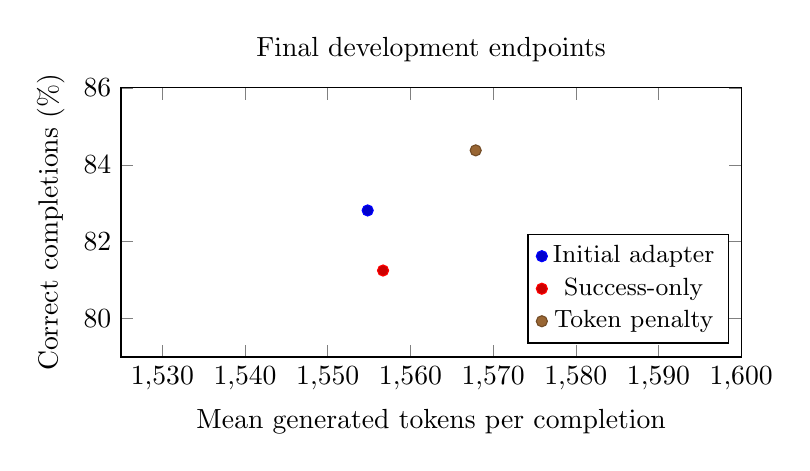
\begin{tikzpicture}
\begin{axis}[width=.78\linewidth,height=5cm,xmin=1525,xmax=1600,ymin=79,ymax=86,
xlabel={Mean generated tokens per completion},ylabel={Correct completions (\%)},legend style={font=\small,at={(.98,.05)},anchor=south east},title={Final development endpoints}]
\addplot+[only marks,mark=*] coordinates {(1554.828125,82.8125)};\addlegendentry{Initial adapter}
\addplot+[only marks,mark=*] coordinates {(1556.6875,81.25)};\addlegendentry{Success-only}
\addplot+[only marks,mark=*] coordinates {(1567.890625,84.375)};\addlegendentry{Token penalty}
\end{axis}\end{tikzpicture}
\par\smallskip
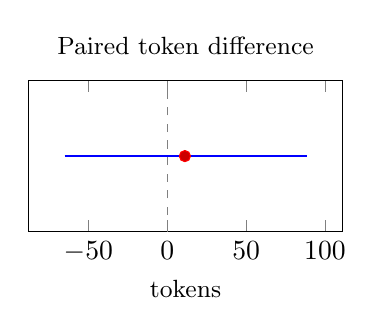
\begin{tikzpicture}
\begin{axis}[width=.46\linewidth,height=3.5cm,xmin=-88.109375,xmax=111.359375,ymin=-1,ymax=1,ytick=\empty,
xlabel={tokens},title={Paired token difference},title style={font=\small},label style={font=\small}]
\addplot+[no marks,thick] coordinates {(-65.09375,0) (88.34375,0)};
\addplot+[only marks,mark=*] coordinates {(11.203125,0)};
\addplot+[no marks,dashed,gray] coordinates {(0,-1) (0,1)};
\end{axis}\end{tikzpicture}
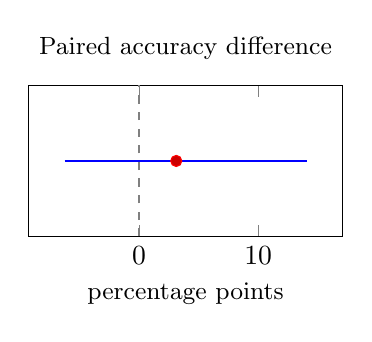
\begin{tikzpicture}
\begin{axis}[width=.46\linewidth,height=3.5cm,xmin=-9.296875,xmax=17.109375,ymin=-1,ymax=1,ytick=\empty,
xlabel={percentage points},title={Paired accuracy difference},title style={font=\small},label style={font=\small}]
\addplot+[no marks,thick] coordinates {(-6.25,0) (14.0625,0)};
\addplot+[only marks,mark=*] coordinates {(3.125,0)};
\addplot+[no marks,dashed,gray] coordinates {(0,-1) (0,1)};
\end{axis}\end{tikzpicture}
\caption{Audited October 10 development comparison, one seed and reused control. Points are final means, not a frontier. Lower panels show penalty-minus-control differences with descriptive 95\% paired task intervals, excluding training-seed and design-selection uncertainty. Both intervals include zero.}
\label{fig:final-outcomes}
\end{figure}
\begin{figure}[htbp]\centering
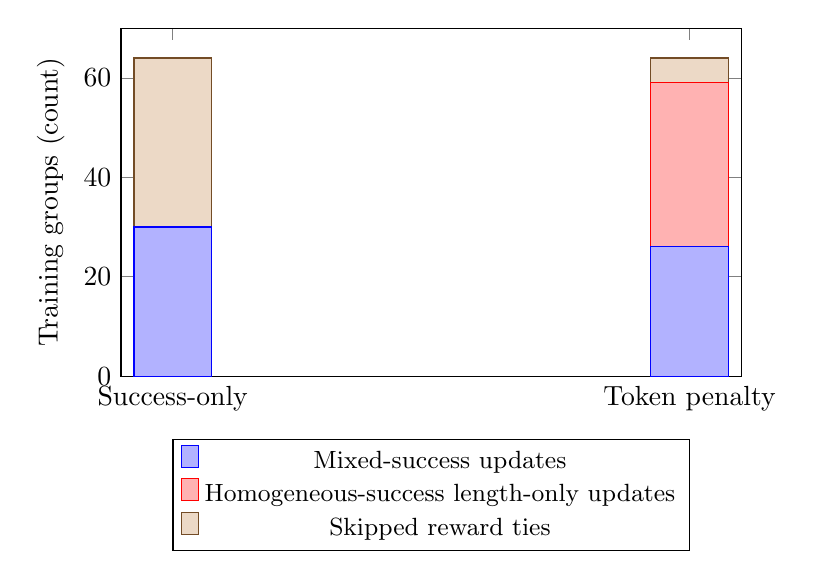
\begin{tikzpicture}
\begin{axis}[ybar stacked,width=.78\linewidth,height=6cm,bar width=28pt,ymin=0,ymax=70,
symbolic x coords={Success-only,Token penalty},xtick=data,ylabel={Training groups (count)},
legend style={font=\small,at={(.5,-.18)},anchor=north,legend columns=1}]
\addplot+ coordinates {(Success-only,30) (Token penalty,26)};\addlegendentry{Mixed-success updates}
\addplot+ coordinates {(Success-only,0) (Token penalty,33)};\addlegendentry{Homogeneous-success length-only updates}
\addplot+ coordinates {(Success-only,34) (Token penalty,5)};\addlegendentry{Skipped reward ties}
\end{axis}\end{tikzpicture}
\caption{Retrospective reconstruction from all 64 groups per arm. Success-only updates on 30 mixed-success groups and skips 34 ties. The penalty updates on 26 mixed-success groups and 33 homogeneous-success groups with varying lengths, skipping five ties. Both arms receive 256 trajectories. These categories explain update support on recorded samples, not a causal performance effect.}
\label{fig:update-support}
\end{figure}
\begin{figure}[htbp]\centering
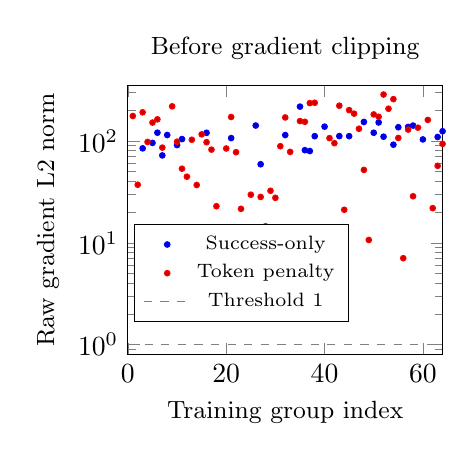
\begin{tikzpicture}
\begin{axis}[width=.46\linewidth,height=5cm,ymode=log,xmin=0,xmax=64,ymin=.8,ymax=350,
xlabel={Training group index},ylabel={Raw gradient L2 norm},label style={font=\small},
legend style={font=\scriptsize,at={(.02,.12)},anchor=south west},title={Before gradient clipping},title style={font=\small}]
\addplot+[only marks,mark=*,mark size=1pt] coordinates {(3,84.42135620117188) (5,95.44694519042969) (6,120.23334503173828) (7,72.0145492553711) (8,114.14982604980469) (10,90.87895202636719) (11,104.08612060546875) (16,119.95144653320312) (21,106.43926239013672) (26,141.38241577148438) (27,58.951622009277344) (32,113.98881530761719) (35,216.69314575195312) (36,81.04090881347656) (37,79.491943359375) (38,111.17473602294922) (40,137.8206024169922) (43,111.36615753173828) (45,111.25066375732422) (48,153.3018341064453) (50,120.10366821289062) (51,151.57086181640625) (52,109.88016510009766) (54,91.70970153808594) (55,136.0893096923828) (57,137.1459197998047) (58,141.20797729492188) (60,103.31727600097656) (63,109.11412811279297) (64,124.30481719970703)};\addlegendentry{Success-only}
\addplot+[only marks,mark=*,mark size=1pt] coordinates {(1,175.33499145507812) (2,37.10155487060547) (3,190.5676727294922) (4,97.61624908447266) (5,151.17578125) (6,162.58181762695312) (7,85.84644317626953) (9,218.231201171875) (10,98.05777740478516) (11,53.31364059448242) (12,44.4913215637207) (13,102.56694030761719) (14,36.894378662109375) (15,115.82779693603516) (16,97.00474548339844) (17,82.03770446777344) (18,22.8486385345459) (19,2.49432635307312) (20,84.1688461303711) (21,171.45753479003906) (22,77.42999267578125) (23,21.522180557250977) (24,4.6230316162109375) (25,29.623048782348633) (27,28.170635223388672) (28,14.513086318969727) (29,32.378787994384766) (30,27.618513107299805) (31,88.60360717773438) (32,169.7086181640625) (33,77.96935272216797) (35,156.31980895996094) (36,153.76429748535156) (37,234.6125030517578) (38,236.47215270996094) (39,7.456293106079102) (41,106.39286041259766) (42,94.95530700683594) (43,221.3907928466797) (44,21.07256317138672) (45,200.3623046875) (46,185.01156616210938) (47,131.48194885253906) (48,51.889801025390625) (49,10.655381202697754) (50,181.753173828125) (51,172.34921264648438) (52,284.7997741699219) (53,206.70660400390625) (54,256.66522216796875) (55,106.8235855102539) (56,7.061657428741455) (57,129.02964782714844) (58,28.616300582885742) (59,134.67555236816406) (61,160.50592041015625) (62,21.872970581054688) (63,56.929691314697266) (64,93.42109680175781)};\addlegendentry{Token penalty}
\addplot+[no marks,dashed,gray] coordinates {(0,1) (64,1)};\addlegendentry{Threshold 1}
\end{axis}\end{tikzpicture}
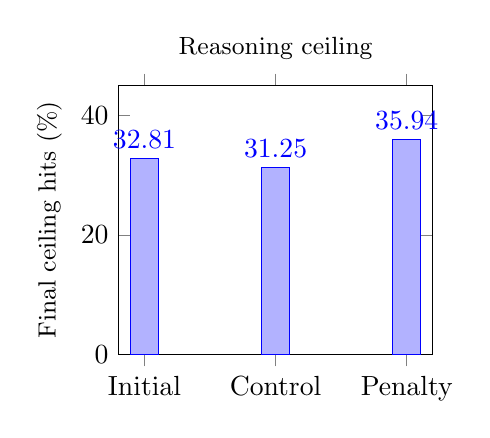
\begin{tikzpicture}
\begin{axis}[ybar,width=.46\linewidth,height=5cm,ymin=0,ymax=45,
symbolic x coords={Initial,Control,Penalty},xtick=data,ylabel={Final ceiling hits (\%)},label style={font=\small},
title={Reasoning ceiling},title style={font=\small},nodes near coords]
\addplot+ coordinates {(Initial,32.8125) (Control,31.25) (Penalty,35.9375)};
\end{axis}\end{tikzpicture}
\caption{Retrospective clipping and ceiling diagnostics from the audited records. Left: all 89 active updates exceed raw gradient norm 1; the vertical axis is logarithmic and clipping precedes Adam. Right: final ceiling hits are 21/64 initial, 20/64 control and 23/64 penalty. These observations do not identify a cause for the final cost response.}
\label{fig:clipping-ceilings}
\end{figure}
% END GENERATED MEASURED FIGURES

\section{Continuation and prospective confirmation}

The \href{https://github.com/arpjw/reward-paper/blob/paper-v1.0.0/docs/REWARD_CONTINUATION.md}{continuation protocol} reuses the verified initial/control evidence and restarts the missing cost-penalty arm from its original initialization. Operational checkpoints every eight groups preserve adapter, optimizer and random state. Actual CUDA resume equivalence must pass before scientific training. The result is labeled a continuation, with one training seed and reused development data. The first continuation failed exact recovery qualification despite identical saved sample rows, with tiny differences in updated adapter and optimizer tensors. A second attempt enables strict deterministic CUDA algorithms before model loading; the exact equality gate remains unchanged. This operational change differs from the retained historical control's execution controls and must be disclosed when interpreting the reused-control comparison. The second attempt passed exact recovery qualification, completed all 64 scientific groups and 64 final evaluation records, and passed an independent Python 3.12 audit using its collected frozen source. The collector and a separate local stream restore verified the entire 1,025,274,422-byte encrypted archive before the final closeout audit. Exact GPU deletion was confirmed by independent provider inventory. These checks establish retained evidence integrity and repeatability for the tested restart; they do not establish a learning benefit.

This contrast did not meet the frozen promising-response rule. A separate prospective mechanism proposal tests whether homogeneous-success cost advantages contribute to a reproducible token response. It calls for fresh matched controls, identical deterministic runtimes, three new training seeds and untouched evaluation tasks. One diagnostic arm masks homogeneous-success groups; this changes the estimator and is explicitly an optimizer intervention, not an unbiased gradient of the original utility. The proposal is unexecuted and requires its own reviewed budget, completed runtime gates and protocol freeze. Adaptive-controller comparisons remain a later possibility. No final-test outcome may select reward scales, prompts, seeds, horizons or checkpoints, and the completed run is not extended.

\section{Limitations}

The synthetic candidate-selection task is a limited proxy for coding. The current development split has been inspected repeatedly during model, prompt and reward design. One seed cannot quantify optimization variability. Tokens measure generated length, not wall-clock cost or total provider spending. Reasoning ceilings and constrained readout change the action space. An arbitrary initial penalty is not a measured Pareto tangent. A future adaptive effect at one effort condition does not establish an entire Pareto frontier.

Two cloud interruptions required a missing-arm continuation; the fixed-reward comparison is now complete. An October 9 provider reply attributes both deletions to account API-key requests through the API/SDK, ruling out provider infrastructure, machine issues, balance exhaustion and template TTL. The responsible key and calling process remain unidentified. The user authorized disabling all previously active API keys and resuming through fresh isolated study access. The \href{https://github.com/arpjw/reward-paper/blob/paper-v1.0.0/docs/REWARD_CONTINUATION_RUN.md}{continuation run log} records its approved \$10 cap, credential mitigation and completed continuation. The support investigation remains open. Recovery and numerical validation support evidence integrity but do not establish a performance improvement.

\section{Reproducibility and release}

The public research release, \href{https://github.com/arpjw/reward-paper/tree/paper-v1.0.0}{\texttt{arpjw/reward-paper}, version \texttt{paper-v1.0.0}}, contains the protocols, derivations, frozen implementation, raw scientific records and source/evidence hashes needed to reconstruct the recorded analysis. The post hoc analysis script checks each used raw input against the public evidence manifest and reconstructs rewards, advantages, update categories and evaluation endpoints on CPU without loading a model. A release manifest distinguishes byte-preserved scientific inputs from report copies sanitized for public presentation. The \href{https://aryasomu.com/papers/reward-contrast/}{website companion} presents the measured plots, group inspector and four fixed-rule development example pairs. Full recorded training and evaluation traces are available in the public scientific subset. No checkpoint performance trajectories or training-seed variability plots are available from this one-seed final-only evaluation. Larger adapter, optimizer and RNG tensors, complete encrypted operational archives, private account records and original Git history remain private. The public analysis reconstruction is distinct from the historical full tensor/restart audit; it does not claim that readers can regenerate that audit from the public subset alone. No prospective sealed final-test data are included.

\section{Conclusion}

In this completed exploratory setting, adding a token penalty creates advantage variation in otherwise tied groups and results in more optimizer updates, while failing to demonstrate token savings at the registered horizon. The penalty scores two more of 64 completions correctly and uses 11.20 more tokens on average; both principal descriptive task intervals include zero. The identical first group demonstrates an estimator mechanism, and the full records show persistent ceilings and universal clipping of active updates. These observations motivate a distinct prospective mechanism study, but they neither identify the cause of the endpoint nor establish adaptive reward superiority. The result is bounded by one seed, a reused inspected development split and a runtime difference. Mathematical derivations, negative findings, exact recovery qualification and retained evidence support a reproducible account of what was tested, rather than a guarantee of behavioral steering.

\appendix
\section{Full gradient through computation history}
\label{sec:cachegradient}

Equation~\eqref{eq:logtrajectory} requires every scratch conditional's parameter gradient. A cached autoregressive computation can be written as
\begin{equation}
 h_0=P_\theta(x),\qquad h_{k+1}=F_k(h_k,\theta),\qquad
 \mathcal L_{\mathrm{scratch}}=a\sum_{k=0}^{B-1}l_k(h_k,\theta),
\end{equation}
where $l_k$ is a block's log likelihood for fixed recorded tokens, and $a=-A_i/G$ is its detached scalar coefficient. Blocks summarize the computation graph, not independently sampled actions. Here $h_k$ is an internal computational state, distinct from the trajectory score $h_\theta$ in Section~\ref{sec:training}. Define the remaining loss as a function of the current state:
\begin{equation}
 \Phi_B(h_B,\theta)=0,\qquad
 \Phi_k(h_k,\theta)=a\,l_k(h_k,\theta)
                    +\Phi_{k+1}(F_k(h_k,\theta),\theta).
\end{equation}
At a state boundary, $d_k=\nabla_{h_k}\Phi_k$ collects the future-loss dependence on that state. The chain rule applied to the second term multiplies its downstream gradient $d_{k+1}$ by the transpose of the state-transition Jacobian $\partial_{h_k}F_k$. The direct parameter branch of the same transition contributes $(\partial_\theta F_k)^\top d_{k+1}$. Adding each local likelihood branch gives
\begin{align}
 d_B&=0,\\
 d_k&=a\,\partial_{h_k}l_k+(\partial_{h_k}F_k)^\top d_{k+1},\label{eq:cachecotangent}\\
 g_k&=a\,\partial_\theta l_k+(\partial_\theta F_k)^\top d_{k+1},\\
 \nabla_\theta\mathcal L_i&=\sum_kg_k+(\partial_\theta P_\theta(x))^\top d_0
             +a\,\nabla_\theta\log p^{\mathcal A}_{\theta,T}(a_i^{\mathrm{ans}}\mid r(x,Z_i)).
 \label{eq:fullhistorygradient}
\end{align}
The readout is a separate re-encoded computation graph. Its parameter gradient is added separately; it does not supply a cotangent to the scratch cache through a discrete decode operation. Setting intermediate $d_k$ to zero would discard history terms and would be truncated backpropagation, a different estimator.
The terminal condition $d_B=0$ follows because no scratch loss remains after the last block. Summing $g_k$ counts the direct parameter branches at every block, while $(\partial_\theta P_\theta(x))^\top d_0$ accounts for parameter dependence in the initial prompt computation. These are all branches of the scratch graph; adding the separate answer gradient completes the per-trajectory loss derivative.

The historical MLX implementation explicitly propagated cache-boundary cotangents. The current CUDA implementation uses a full teacher-forced scratch graph with activation checkpointing and a separate readout backward pass. Recomputing activations can reduce memory while retaining the chain rule, provided it reproduces the same computation. Numerical replay tolerances quantify observed approximation, not an analytic equality certificate for every gradient. Results from distinct numerical backends are not pooled as if their policies were identical.

\section{Checkpoint state, exact recovery and durable evidence}
\label{sec:recovery}

A recoverable state contains more than adapter weights. Write
\begin{equation}
 \mathcal S_k=(\theta_k,m_k,v_k,t_k,k,\mathcal R_k,\mathcal P_k,\mathcal I),
\end{equation}
where $t_k$ is the optimizer's update count, $k$ is the completed group position, $\mathcal R_k$ contains Python, NumPy and Torch CPU/CUDA random states, $\mathcal P_k$ authenticates record prefixes and named parameter ordering, and $\mathcal I$ binds source, inputs, task schedule, sampling seeds and runtime. The optimizer's per-parameter step state is preserved. A notional update transition is
\begin{equation}
 (\mathcal S_{k+1},\mathcal O_{k+1})=F_{\omega,k}(\mathcal S_k),
\end{equation}
where $\omega$ includes the generating runtime and numerical-kernel controls, and $\mathcal O$ denotes sampled records and update metrics. A deterministic transition is an assumption about execution controls, not a consequence of recording seeds alone.

The mandatory CUDA qualification saves state after the first prescribed group, computes group two uninterrupted, reloads group-one state into a fresh model and optimizer, then repeats group two. It requires
\begin{align}
 \mathcal O_2^{\mathrm{uninterrupted}}&=\mathcal O_2^{\mathrm{reloaded}},\\
 \theta_2^{\mathrm{uninterrupted}}&=\theta_2^{\mathrm{reloaded}},\\
 (m_2,v_2,t_2,\mathcal R_2)^{\mathrm{uninterrupted}}
    &=(m_2,v_2,t_2,\mathcal R_2)^{\mathrm{reloaded}}.
\end{align}
Adapter serialization hashes must match; optimizer/RNG structures and tensors are compared exactly. Both prescribed updates must be nonzero. The qualification's repeated trajectories are not added to scientific training.

The first continuation failed this exact test: sample rows matched, but small adapter/optimizer differences remained. The second uses strict deterministic CUDA controls and passed the unchanged test. This establishes repeatability for the tested restart on its recorded runtime. It does not prove bitwise equivalence for every future restart, another architecture or another backend. The retained success-only control did not use the new bootstrap controls; that operational difference limits the reused-control contrast.

Scientific checkpoints at $k\in\{0,8,16,\ldots,64\}$ bind the adapter, optimizer, random state and exact prefix. Every completed group and paired evaluation task is protected by an immutable recovery manifest before the next unit of work. For each included file $f$, retain
\begin{equation}
 \mathcal M[f]=\bigl(\operatorname{SHA256}(f),\operatorname{bytes}(f)\bigr).
\end{equation}
The encrypted off-Pod object is read back in full and checked against both fields. An acknowledgement must bind the same Pod ID, source freeze, sequence and manifest hash. Missing or mismatched acknowledgement blocks further sampling. A saved weight file without optimizer state or a verified record prefix is not a qualified resume point. An archived partial result does not constitute a completed comparison.

\section{What is established and what remains empirical}

The mathematical statements in this draft have distinct scopes:
\begin{enumerate}
 \item Equations~\eqref{eq:constrained}--\eqref{eq:lambdabeta} give an exact algebraic scalarization for interior weights with positive, fixed baseline references.
 \item Equations~\eqref{eq:mirror}--\eqref{eq:controller} solve a strictly convex one-dimensional dual step while treating gain estimates as fixed. They do not prove convergence of the coupled learning process.
 \item Equation~\eqref{eq:loo} is conditionally unbiased under independent current-policy samples, fixed penalty and exact scores. Clipping, Adam, finite precision and a changing penalty prevent interpreting every parameter update as that ideal expectation.
 \item Equations~\eqref{eq:replaygates}--\eqref{eq:lossgate} and the exact restart check are implemented numerical gates. Passing them supports evidence integrity, not a success-cost improvement.
 \item Equation~\eqref{eq:bootstrapinterval} describes the frozen one-seed development analysis. It does not quantify training-seed variation or remove repeated development selection.
 \item The fixed-reward development comparison is complete and independently audited. Its cost and accuracy differences are small or uncertain. A reliable reward response, an adaptive-rule advantage and a Pareto-frontier claim require increasingly broader empirical evidence; none of those stronger claims is established here.
\end{enumerate}
The full derivation and experiment-specific qualifications are also preserved in \href{https://github.com/arpjw/reward-paper/blob/paper-v1.0.0/MATH.md}{MATH.md}, the \href{https://github.com/arpjw/reward-paper/blob/paper-v1.0.0/docs/CAPABILITY_RL_METHOD.md}{historical RL method}, the \href{https://github.com/arpjw/reward-paper/blob/paper-v1.0.0/docs/REWARD_CONTRAST_METHOD.md}{fixed-contrast protocol} and the \href{https://github.com/arpjw/reward-paper/blob/paper-v1.0.0/docs/REWARD_CONTINUATION_RUN.md}{current run log}. Preparation status in a historical protocol is not a current execution receipt.

\begin{thebibliography}{99}
\bibitem{rloo} Arash Ahmadian et al.
\href{https://arxiv.org/abs/2402.14740}{Back to Basics: Revisiting REINFORCE Style Optimization for Learning from Human Feedback in LLMs}. arXiv:2402.14740, 2024.
\bibitem{dler} Shih-Yang Liu et al.
\href{https://arxiv.org/abs/2510.15110}{DLER: Doing Length pEnalty Right: Incentivizing More Intelligence per Token via Reinforcement Learning}. arXiv:2510.15110, 2025.
\bibitem{anish} Anish Lakkapragada.
\href{https://anishlk.com/swe-2-extended/}{Extending SWE-2's reward function to steer the Pareto frontier}. 2026.
\bibitem{swe} Cognition.
\href{https://cognition.com/blog/swe-2}{Introducing SWE-2: Pushing the Pareto Frontier}. 2026.
\bibitem{reinforce} Ronald J. Williams.
\href{https://link.springer.com/article/10.1007/BF00992696}{Simple statistical gradient-following algorithms for connectionist reinforcement learning}.
\emph{Machine Learning}, 8:229--256, 1992.
\bibitem{lora} Edward J. Hu et al.
\href{https://arxiv.org/abs/2106.09685}{LoRA: Low-Rank Adaptation of Large Language Models}. arXiv:2106.09685, 2021.
\bibitem{adam} Diederik P. Kingma and Jimmy Ba.
\href{https://arxiv.org/abs/1412.6980}{Adam: A Method for Stochastic Optimization}. ICLR, 2015.
\bibitem{qwen} Qwen.
\href{https://huggingface.co/Qwen/Qwen3-4B-Instruct-2507}{Qwen3-4B-Instruct-2507 model card}.
\bibitem{evidence} Project evidence:
\href{https://github.com/arpjw/reward-paper/blob/paper-v1.0.0/docs/CAPABILITY_CUDA_RESULTS.md}{CUDA pilot},
\href{https://github.com/arpjw/reward-paper/blob/paper-v1.0.0/docs/COMPACT_REWARD_RESULTS.md}{compact diagnostic},
\href{https://github.com/arpjw/reward-paper/blob/paper-v1.0.0/docs/REWARD_GEOMETRY_DIAGNOSIS.md}{reward geometry}, and
\href{https://github.com/arpjw/reward-paper/blob/paper-v1.0.0/docs/REWARD_CONTRAST_RETRY_INTERRUPTION.md}{recovered retry}.
\end{thebibliography}
\end{document}
